\documentclass{../cssheet}

%--------------------------------------------------------------------------------------------------------------
% Basic meta data
%--------------------------------------------------------------------------------------------------------------

\title{Abstraktion}
\author{Prof. Dr. Christian Spannagel}
\date{\today}
\hypersetup{%
    pdfauthor={\theauthor},%
    pdftitle={\thetitle},%
    pdfsubject={Aufgabenblatt Algebra},%
    pdfkeywords={algebra}
}

%--------------------------------------------------------------------------------------------------------------
% document
%--------------------------------------------------------------------------------------------------------------

\begin{document}
\printtitle

\textbf{Vorbemerkung:}  Ihr dürft gerne ChatGPT oder Google Bard oder eine andere KI verwenden, um mal zu schauen, welche Lösungen euch hier vorgeschlagen werden. Macht das aber erst, \emph{nachdem} ihr selbst eine Lösung gefunden habt! Vergleicht eure Lösung mit der Lösung der KI. Ist die Lösung der KI korrekt? Hat sie eine andere Lösung gefunden als ihr? Wie beurteilt ihr die Qualität der Ausgabe? Lasst die KI gerne auch mehrere Lösungen erzeugen. Vielleicht präsentiert sie euch auch ganz neue Lösungsansätze. 

\textbf{Aufgabe 1 (Was ist Abstraktion?):}  Was ist Abstraktion für euch? Wie würdet ihr jemandem erklären, was Abstraktion ist? Habt ihr ein anschauliches Beispiel für Abstraktion, z.\,B. aus dem Alltag?

\textbf{Aufgabe 2 (Wozu Abstraktion?):} Wozu ist Abstraktion gut?

\textbf{Aufgabe 3 (Mathematical reality):} Lest den Text \glqq{}Reality and Imagination\grqq{} von Paul Lockart (das ist das Vorwort aus seinem Buch \glqq{}Measurement\grqq{}\footnote{Lockart, P. (2012). \emph{Measurement}. Harvard: Harvard University Press}). Diskutiert, was das mit Abstraktion zu tun hat.

\textbf{Aufgabe 4 (Wissenschaft Mathematik):} Die Mathematik ist die Wissenschaft der Muster und Strukturen. Was hat das mit Abstraktion zu tun?

\textbf{Aufgabe 5 (Wimmelbild):} Findet in folgendem Bild alle möglichen Abstraktionen!

\begin{center}
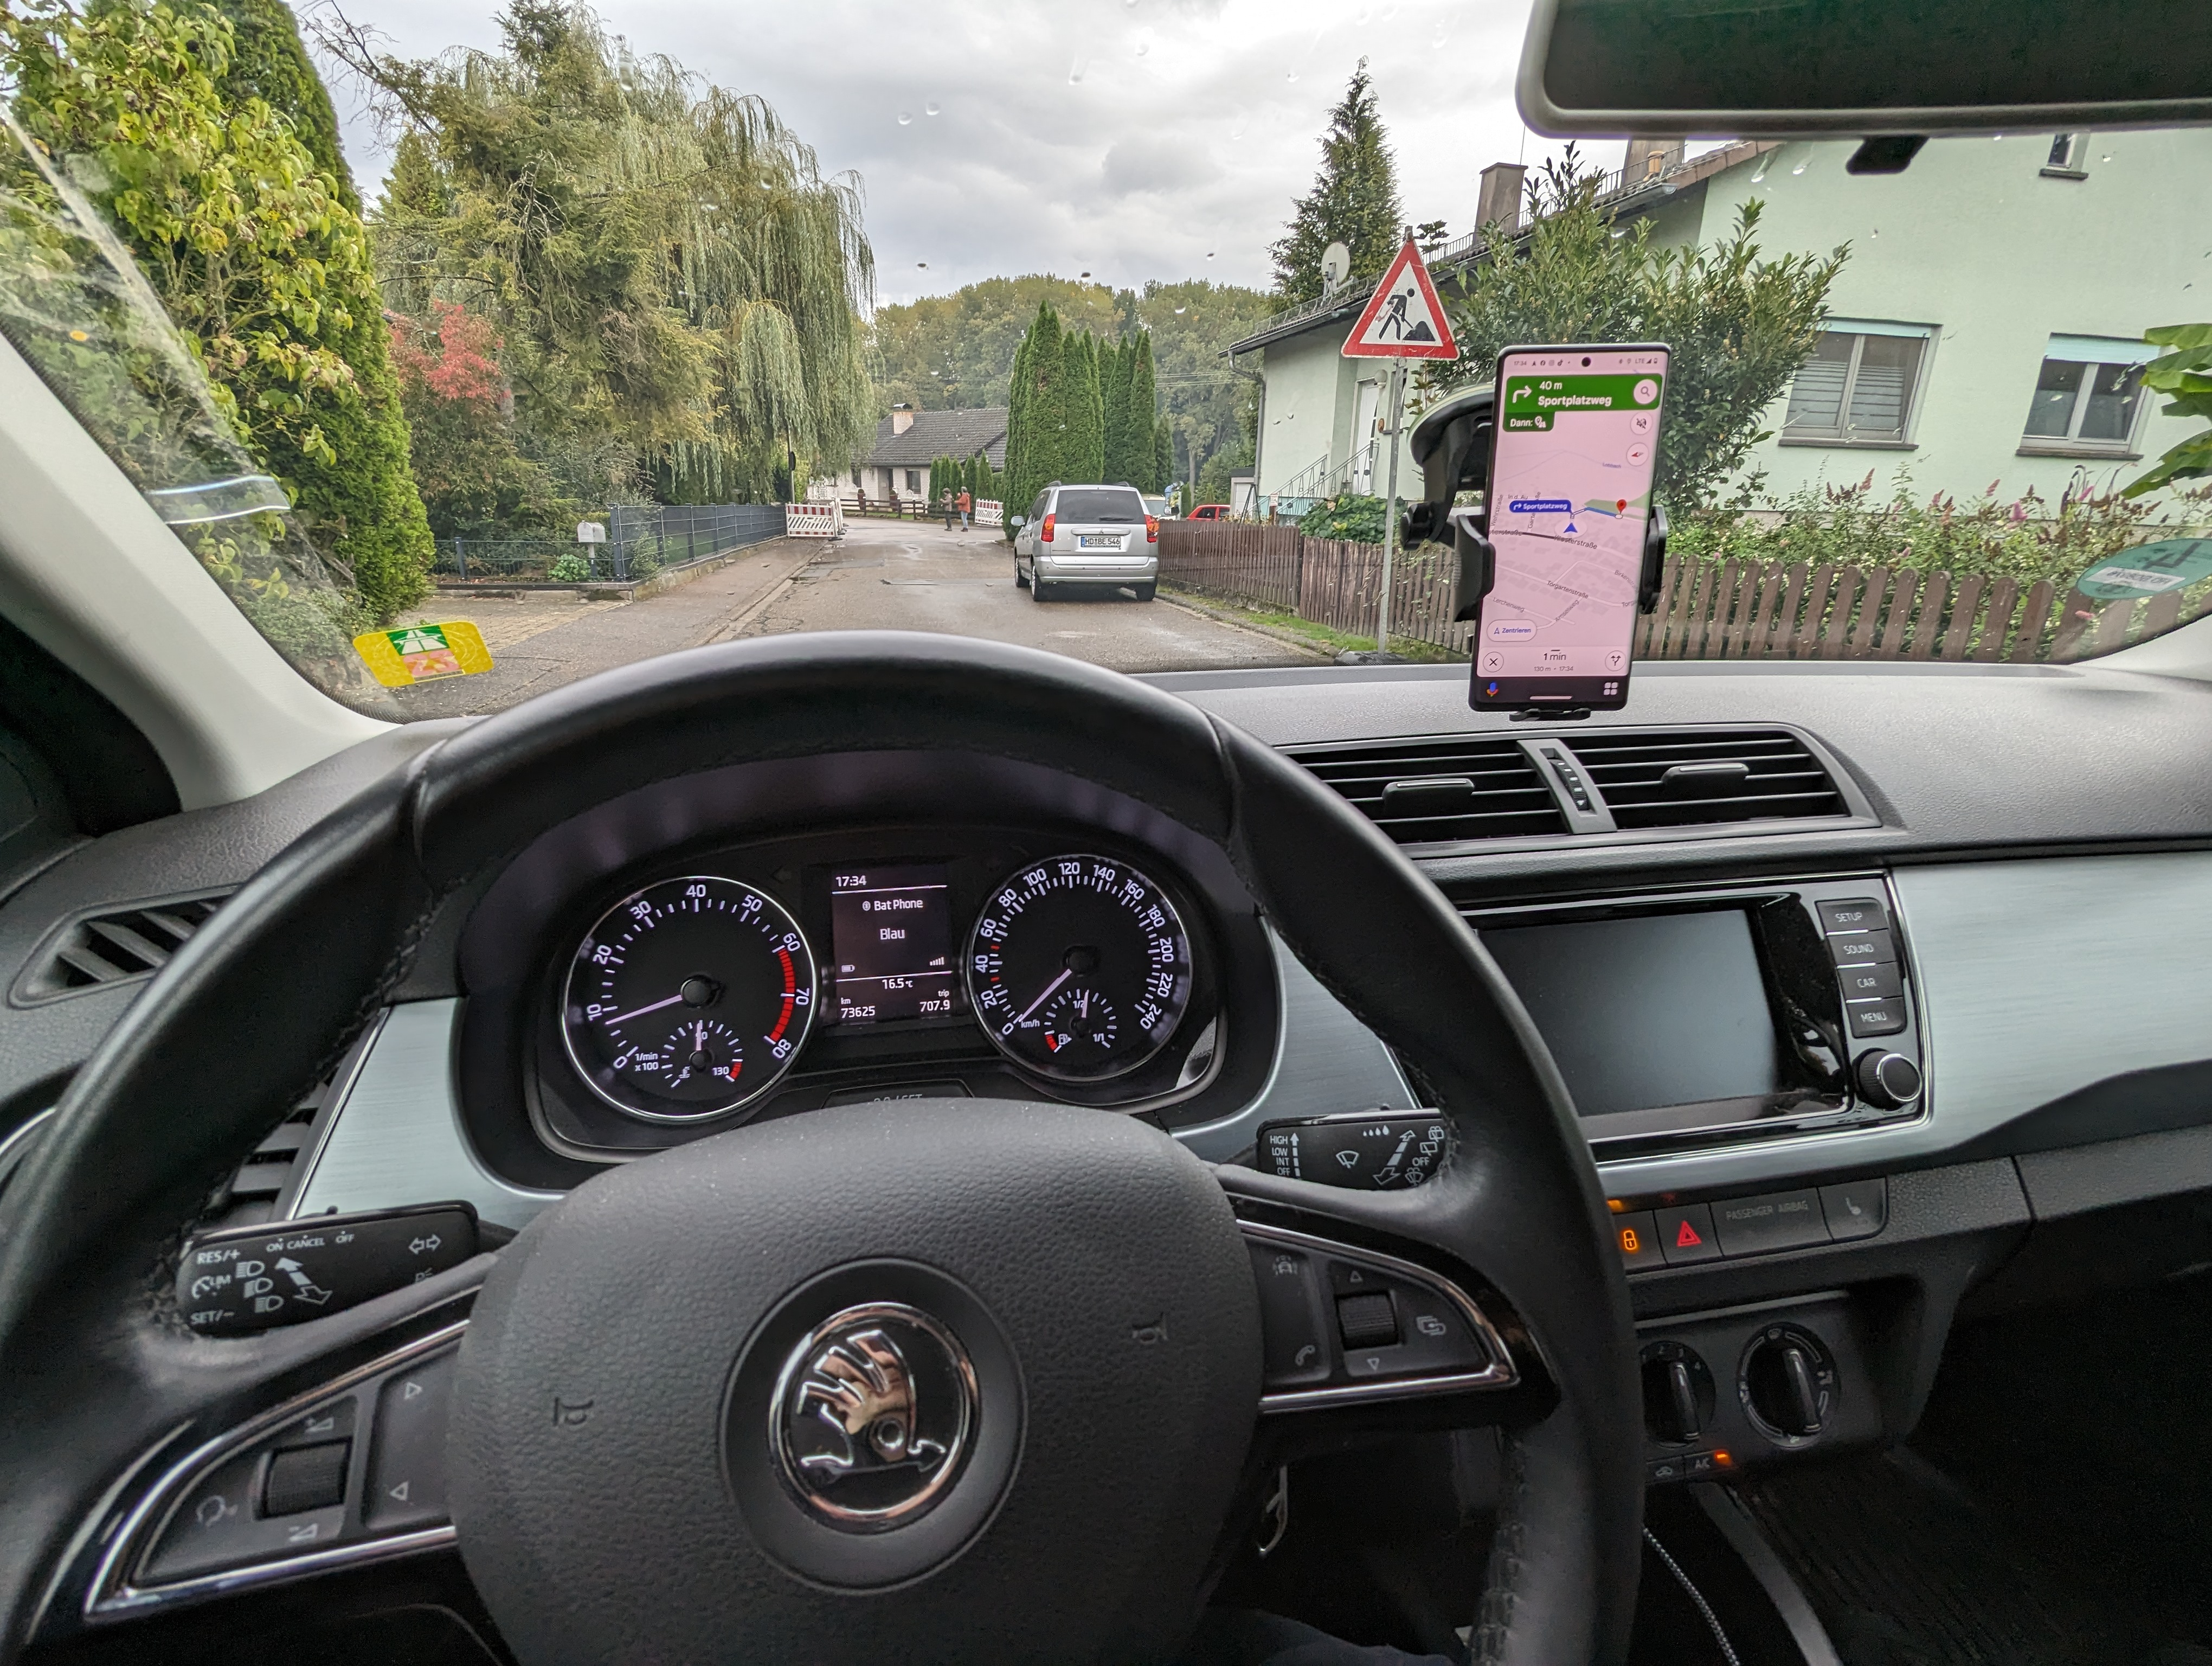
\includegraphics[width=10cm]{cockpit.jpg}
\end{center}


\printlicense

\printsocials


\end{document}
